\documentclass[tikz]{standalone}
\usepackage{bm}
\usepackage{tcolorbox}
\usepackage{mathtools}
\usepackage{pgfplots}
\pgfplotsset{width=7cm,compat=1.8}
\pgfplotsset{%
  colormap={whitered}{color(0cm)=(white);
  color(1cm)=(orange!75!red)}
}


\begin{document}
  
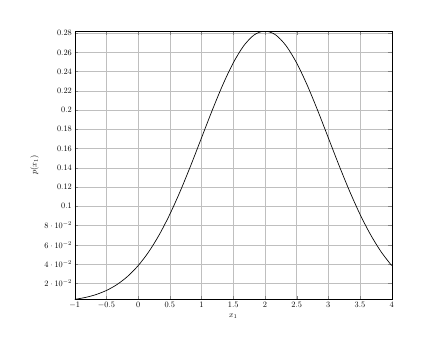
\begin{tikzpicture}[
  scale = 0.3,
  declare function = {mu1=1;},
  declare function = {mu2=2;},
  declare function = {sigma1=0.5;},
  declare function = {sigma2=1;},
  declare function = {normal(\m,\s)=1/(2*\s*sqrt(pi))*exp(-(x-\m)^2/(2*\s^2));},
  declare function = {bivar(\ma,\sa,\mb,\sb)=
    1/(2*pi*\sa*\sb) * exp(-((x-\ma)^2/\sa^2 + (y-\mb)^2/\sb^2))/2;}]
  \begin{axis}[
    colormap name  = whitered,
    width          = 15cm,
    view           = {45}{65},
    enlargelimits  = false,
    grid           = major,
    domain         = -1:4,
    y domain       = -1:4,
    samples        = 26,
    xlabel         = $x_1$,
    ylabel         = $p(x_1)$,
  ]
    \addplot [domain=-1:4,samples=31, thick, smooth]
      (x,{normal(mu2,sigma2)});
  \end{axis}
\end{tikzpicture}


\end{document}
